\documentclass{article}

% Default packages
\usepackage[utf8]{inputenc}
\usepackage[spanish]{babel}
\usepackage{fancyhdr}
\usepackage{tikz}
\usepackage{amssymb}
\usepackage{float}

\usepackage{pdfpages}
\usepackage{listings}
\usepackage{xcolor}

\lstset{
    showstringspaces=false, % don't mark spaces in strings
    numbers=left, % display line numbers on the left
    commentstyle=\color{blue}, % comment color
    keywordstyle=\color{magenta}, % keyword color
    stringstyle=\color{red} % string color
}

\usepackage{color}
\definecolor{lightgray}{rgb}{0.95, 0.95, 0.95}
\definecolor{darkgray}{rgb}{0.4, 0.4, 0.4}
%\definecolor{purple}{rgb}{0.65, 0.12, 0.82}
\definecolor{editorGray}{rgb}{0.95, 0.95, 0.95}
\definecolor{editorOcher}{rgb}{1, 0.5, 0} % #FF7F00 -> rgb(239, 169, 0)
\definecolor{editorGreen}{rgb}{0, 0.5, 0} % #007C00 -> rgb(0, 124, 0)
\definecolor{orange}{rgb}{1,0.45,0.13}		
\definecolor{olive}{rgb}{0.17,0.59,0.20}
\definecolor{brown}{rgb}{0.69,0.31,0.31}
\definecolor{purple}{rgb}{0.38,0.18,0.81}
\definecolor{lightblue}{rgb}{0.1,0.57,0.7}
\definecolor{lightred}{rgb}{1,0.4,0.5}
\usepackage{upquote}
\usepackage{listings}
% JavaScript
\lstdefinelanguage{JavaScript}{
  morekeywords={typeof, new, true, false, catch, function, return, null, catch, switch, var, if, in, while, do, else, case, break},
  morecomment=[s]{/*}{*/},
  morecomment=[l]//,
  morestring=[b]",
  morestring=[b]'
}




\usepackage{graphicx}
\graphicspath{ {./imagenes/} }

\usepackage{geometry}
\geometry{margin=2cm}

\title{Tablero}
\author{Axel Treviño Palacios} 
\date{21 de enero de 2020}
\def\thenumber{6}

\makeatletter
\let\thetitle\@title
\let\theauthor\@author
\let\thedate\@date
\makeatother

\pagestyle{fancy}
\fancyhead{}
\fancyfoot{}
\fancyfoot[R]{\thepage}
\fancyfoot[L]{\thetitle}
\renewcommand{\headrulewidth}{0pt}
\renewcommand{\footrulewidth}{0.5pt}

\begin{document}
	\begin{titlepage}
		\centering	 
	 	
	 	\begin{tikzpicture}[remember picture, overlay]
			\node[anchor=north east,inner sep=1cm] at (current page.north east)
				{
\includegraphics[height=3.5cm]{logoEscom}};
			\node[anchor=north west,inner sep=1cm] at (current page.north west)
				{
\includegraphics[height=3.5cm]{logoPoli}};
		\end{tikzpicture}

		\vspace{4cm}
		{\Large \scshape Instituto Politécnico Nacional \par}
		\vspace{1cm}

		{\rmfamily \bfseries \Large Escuela Superior de Cómputo \par}
		\vspace{4cm}

		{\itshape\Large Práctica \#\thenumber \par}
		\vspace{0.5cm}
		
		{\scshape\Huge \thetitle \par}
		\vspace{5cm}
			
		{\itshape\Large \theauthor \par}
		2CM5
		
		\thedate				
		
		\vfill
	\end{titlepage}

	\section{Objetivo}
	Elaborar un programa implementando con un autómata de pila para reconocer el lenguaje libre de contexto \{ 0 \textsuperscript{n} 1 \textsuperscript{n} | n $>$= 1 \}.

	
	
	\section{Códigos}
	Hay dos archivos, el archivo del servidor y el archivo de cliente.
	
	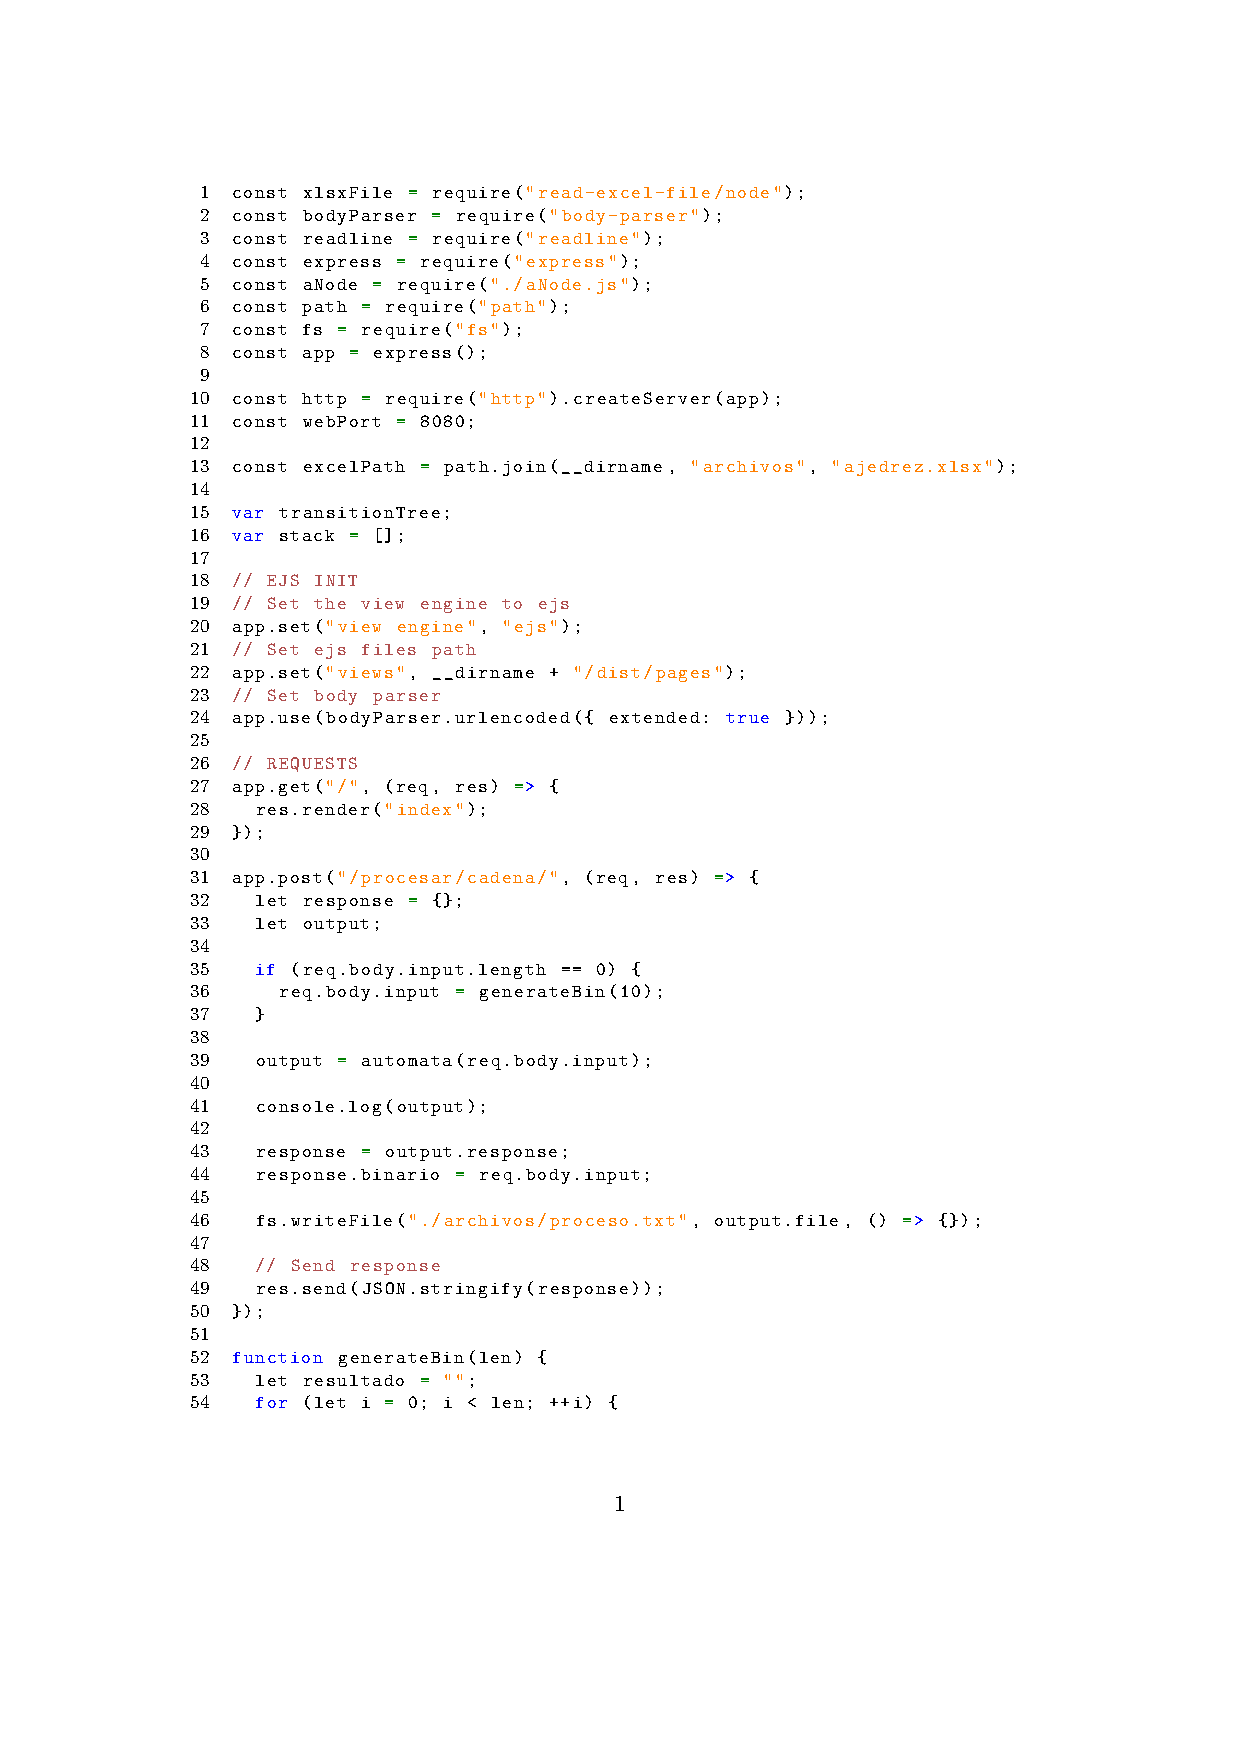
\includepdf[page=-]{servidor.pdf}

	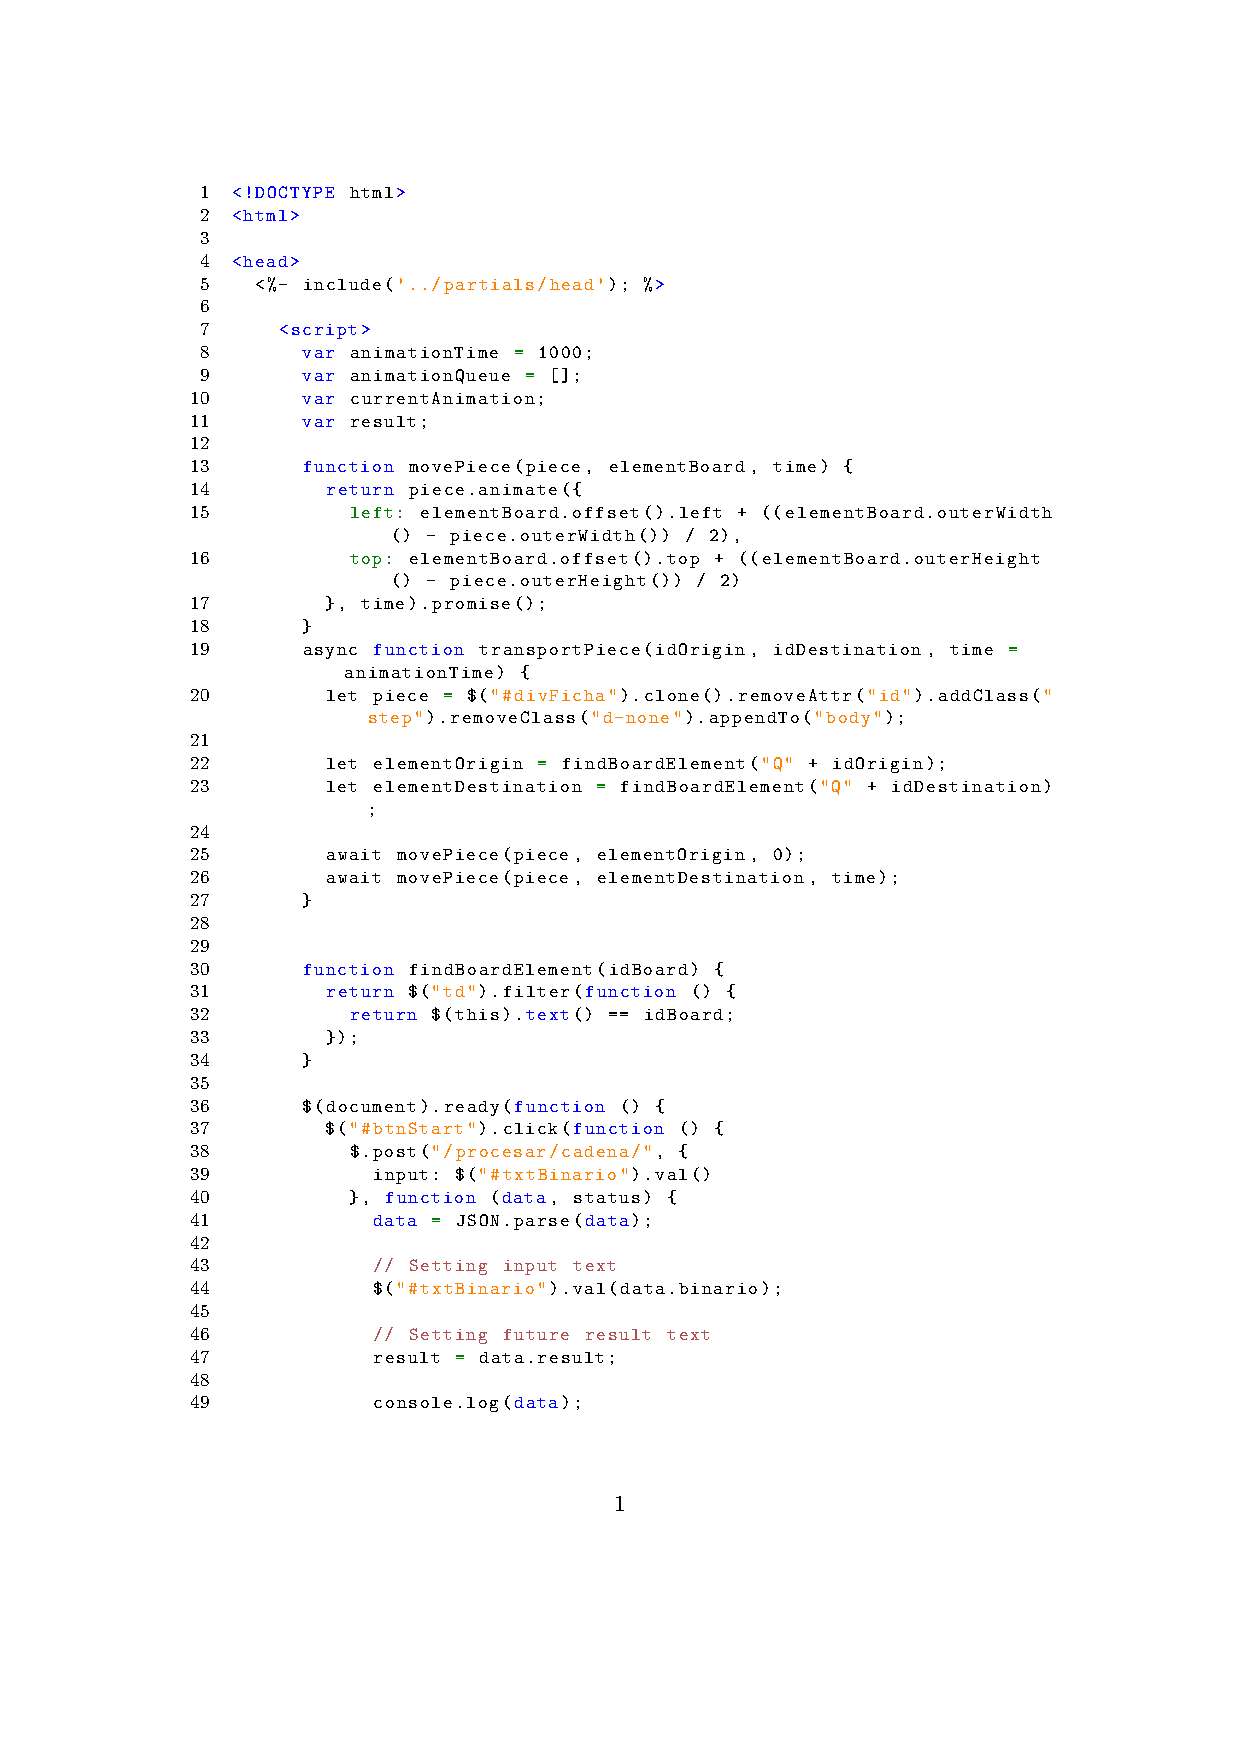
\includepdf[page=-]{cliente.pdf}
	

	\newpage
	\section{Resultados}	
	Autómata ejecutándose:	
	
	\begin{figure}
    \centering
    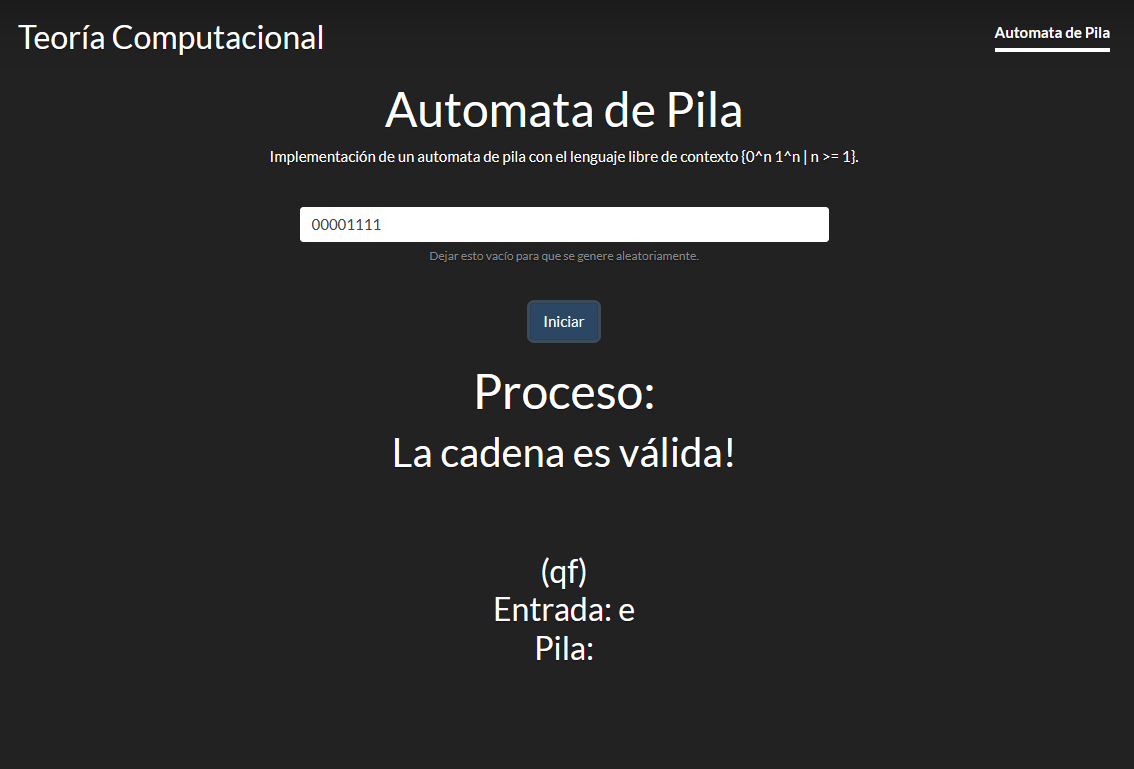
\includegraphics[width=0.75\textwidth]{automata1}
    \caption{Tabla de Conversión}
    \label{fig:proceso}
	\end{figure}

	\begin{figure}
	\centering
    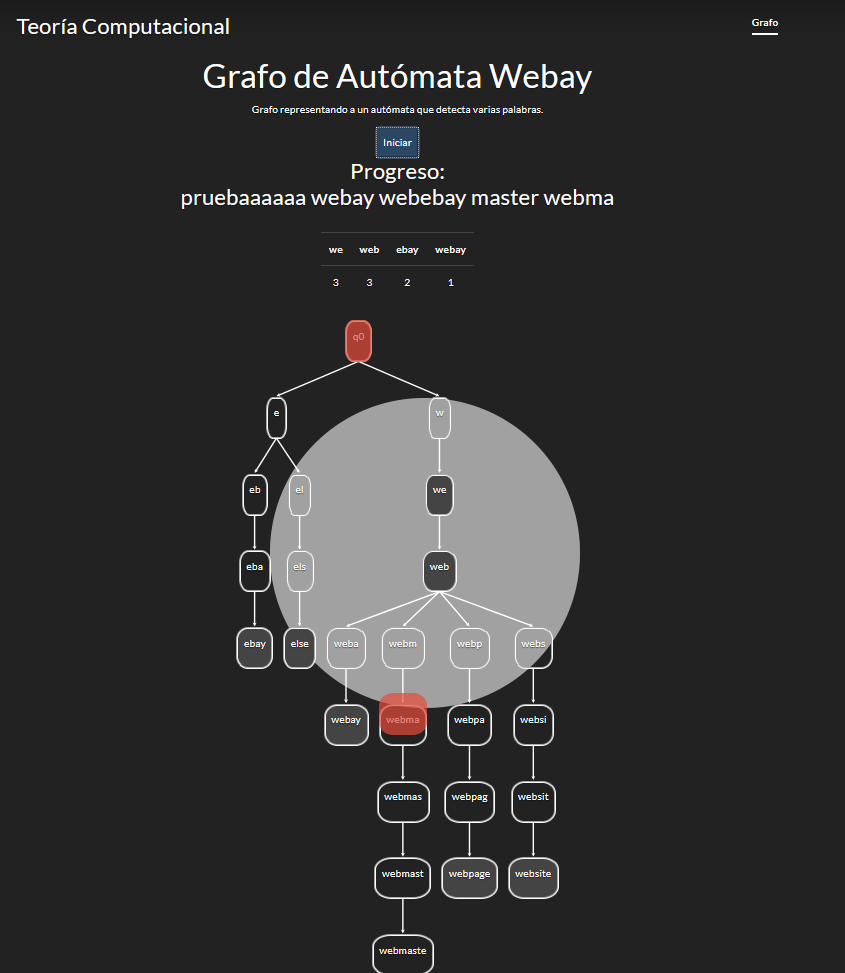
\includegraphics[width=0.75\textwidth]{automata2}
    \caption{Tabla de Conversión}
    \label{fig:proceso}
	\end{figure} 


\end{document}
